\def\dt{\,\text{dt}\,}
\def\dx{\,\text{dx}\,}
\def\dk{\,\text{dk}\,}
\chapter{Vorbereitung}
    \section{Fourierreihen und -transformation}
Die Fourier-Analysis findet gerade in der Optik häufig Anwendung. Im Kontext der 
Holografie stellen vor allem Fourierreihen und die Fouriertransformation nützliche
Hilfsmittel dar, weshalb diese zur Vorbereitung näher betrachtet werden sollen.
    \subsection*{Fourierreihenentwicklung}
Die Fourierreihe bietet die Möglichkeit einen großen Teil der periodischen 
Funktionen durch eine Linearkombination von Sinus- und Kosinustermen verschiedener
Frequenzen und Amplituden zu entwickeln.
        \begin{align*}
           f(t) = \sum_{k=0}^\infty a_k \cos(\omega_k \, t) + b_k \sin(\omega_k \, t) 
           \qquad \text{mit  } \omega_k =  \frac{2 \pi k}{T}
        \end{align*}
$T$ sei hierbei die Periodendauer der Funktion. Die \emph{Fourierkoeffizienten} $a_k$
und $b_k$ werden hier beschrieben durch
        \begin{align*}
            a_0 = \frac{1}{T} \int_{-T/2}^{+T/2} f(t) \dt \quad &a_k = \frac{2}{T}
            \int_{-T/2}^{+T/2} f(t) \cos(\omega_k \, t) \dt \;(k\neq 0)\\
            &b_k = \frac{2}{T} \int_{-T/2}^{+T/2} f(t) \sin()\omega_k \, t) \dt
        \end{align*}
Dies soll nun an zwei wichtigen Funktionen demonstriert werden.
            \subsubsection*{Rechtecksfunktion}
        \begin{wrapfigure}{r}{0.45\textwidth}
            \vspace{10pt}
            \centering
            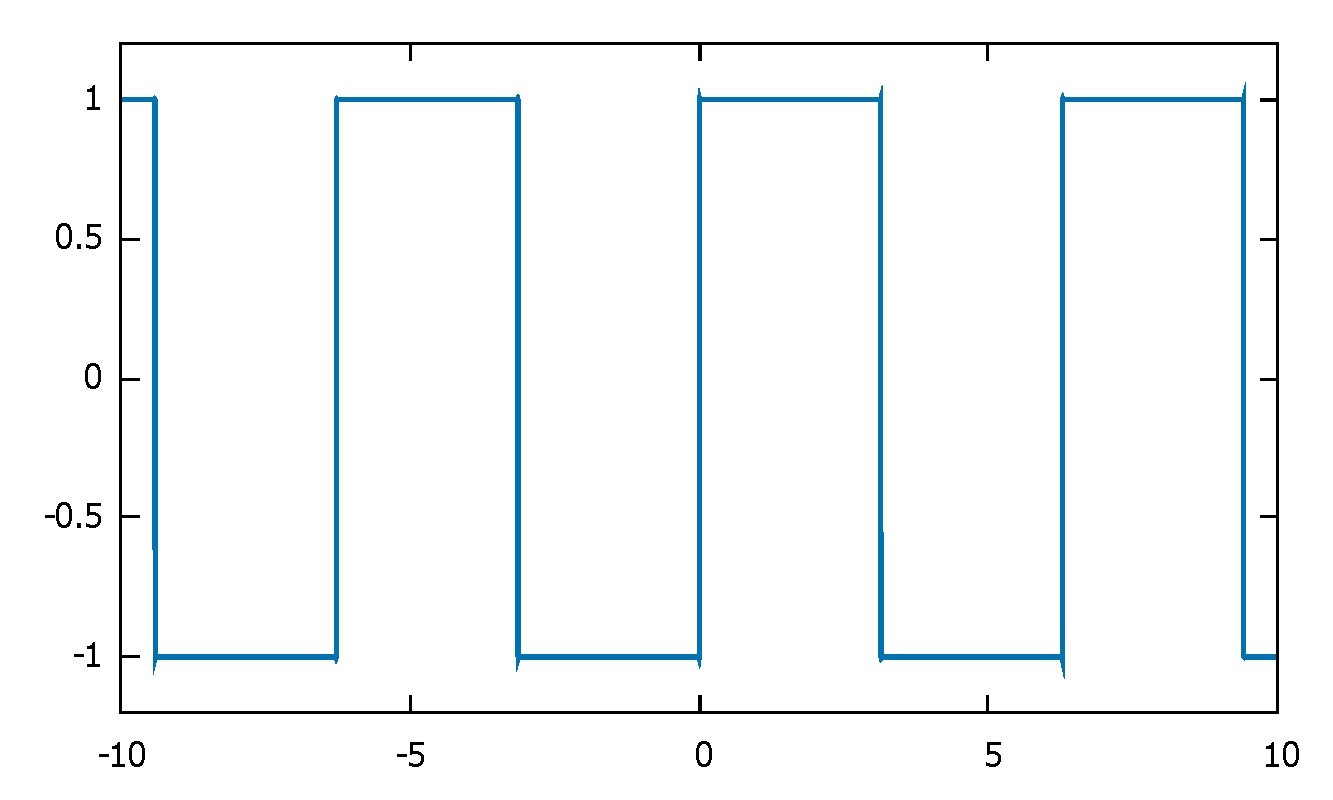
\includegraphics[width=0.4\textwidth]{Abb/rechteck.pdf}
            \caption{Rechtecksfunktion}
            \label{rechteck}
            \vspace{10pt}
        \end{wrapfigure}
Die Rechtecksfunktion ist gegeben durch
        \begin{align*}
            f(t) = \begin{cases}
                -1 & \text{für } -1 < t < 0 \\
                 1 & \text{für }  0 < t < 1
            \end{cases}   
        \end{align*}
mit periodischer Fortsetzung.\\
Um nun die Fourierreihendarstellung nutzen zu können, müssen zuerst die Koeffizienten
errechnet werden. Für $T=2$ ergibt sich:
        \begin{itemize}
            \item da die Rechtecksfunktion eine ungerade Funktion ist gilt $a_k = 0$
            \item für die $b_k$ gilt
                \begin{align*}
                   b_k &=\frac{2}{2} \int_{-1}^{1} f(t) \sin(\pi k t ) \dt = 
                   \int_{-1}^{0} - \sin(\omega_k t) \dt 
                   + \int_0^1 \sin(\omega_k t ) \dt \\
                   &= \frac{1}{\pi k} \left[
                       \left(1 - \cos
                        \left(-\frac{\pi k}{2}
                        \right)
                       \right)
                     + \left(-\cos
                        \left( \frac{\pi k}{2}
                        \right) + 1
                       \right)
                    \right]
                    = \frac{2}{\pi k} \left( 1 + \cos(\pi k)\right)
                \end{align*}
            \end{itemize}
Somit erhalten wir für die Fourierreihenentwicklung der Rechtecksfunktion
                \begin{align*}
                   f(t) = \sum_{k=0}^\infty \frac{2}{\pi k} (1 + \cos(\pi k)) 
                   \sin(\pi k t) 
                \end{align*}
                \begin{figure}[htbp]
                  \begin{minipage}{0.45\textwidth}
                   \centering
                    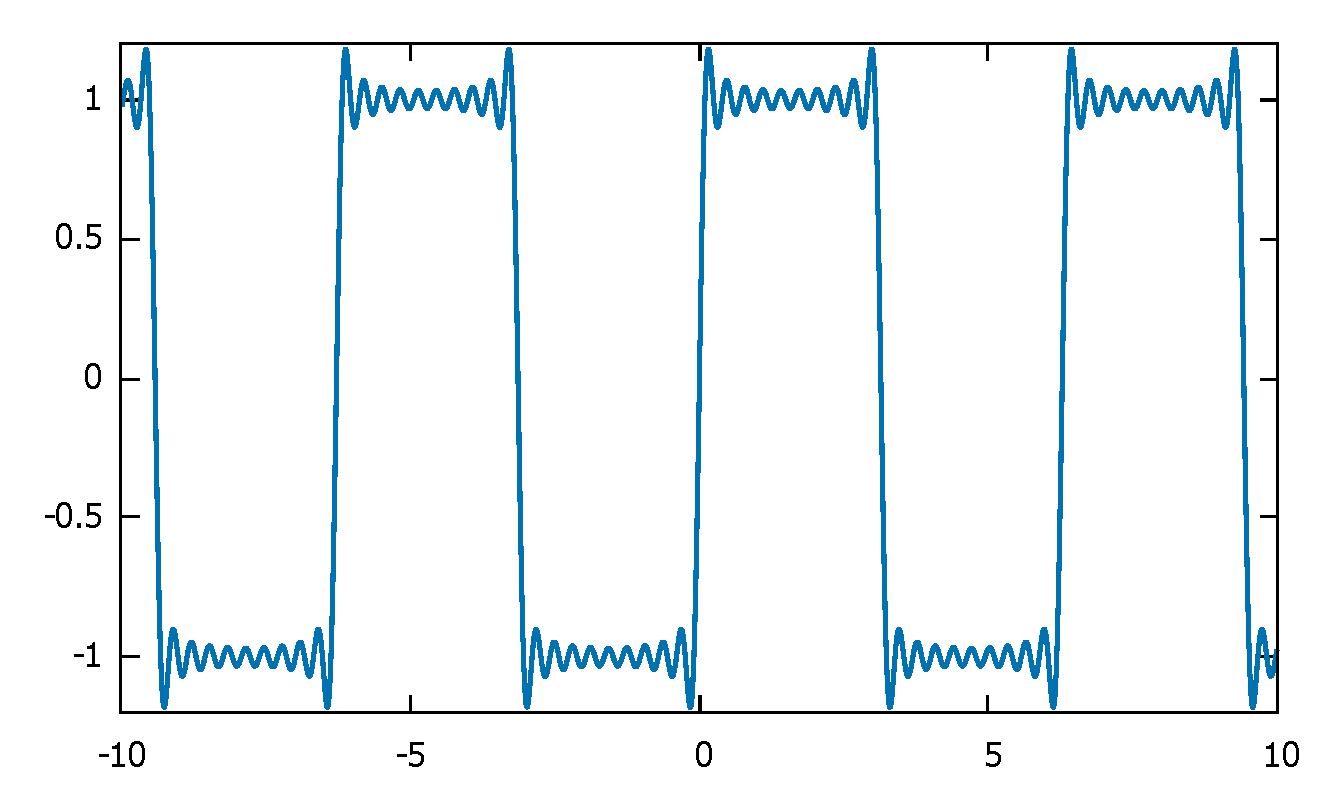
\includegraphics[width=0.9\textwidth]{Abb/rechteck_10}
                    \caption{Die Rechtecksfunktion bis zum 10. Summanden entwickelt}
                    \label{rechteck_10}
                  \end{minipage}\hfill
                  \begin{minipage}{0.45\textwidth}
                   \centering
                    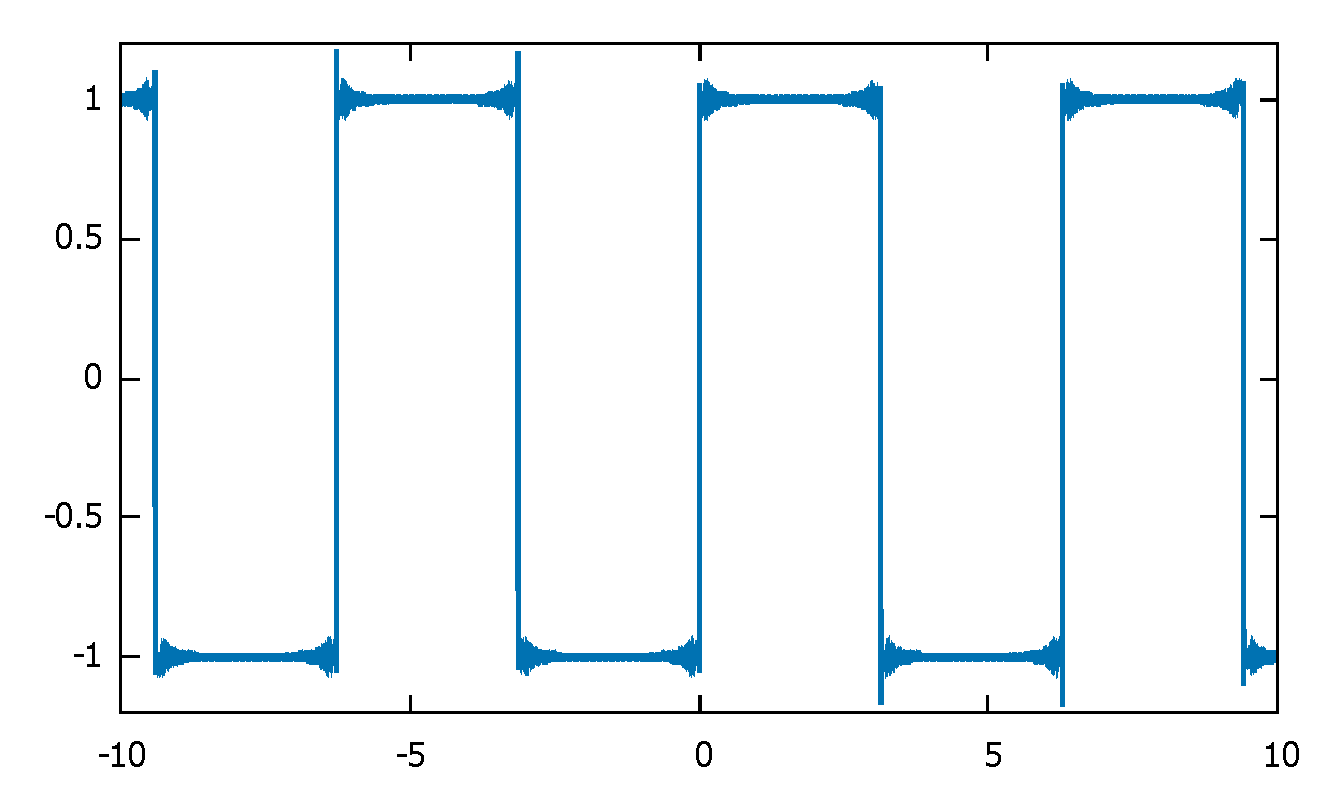
\includegraphics[width=0.9\textwidth]{Abb/rechteck_1000.pdf}
                    \caption{Die Rechtecksfunktion bis zum 1000. Summanden entwickelt}
                    \label{reckteck_1000}
                  \end{minipage}
                \end{figure}
In Abbildung \ref{rechteck} ist die Reihenentwicklung bis zum 100000. Glied 
geplottet, während in Abbildung \ref{rechteck_10} und \ref{reckteck_1000} bis zur 
10. und 1000. Ordnung geplottet wurde. 

                    \subsubsection*{Dreiecksfunktion}
            \begin{wrapfigure}{r}{0.45\textwidth}
                \vspace{10pt}
                \centering
                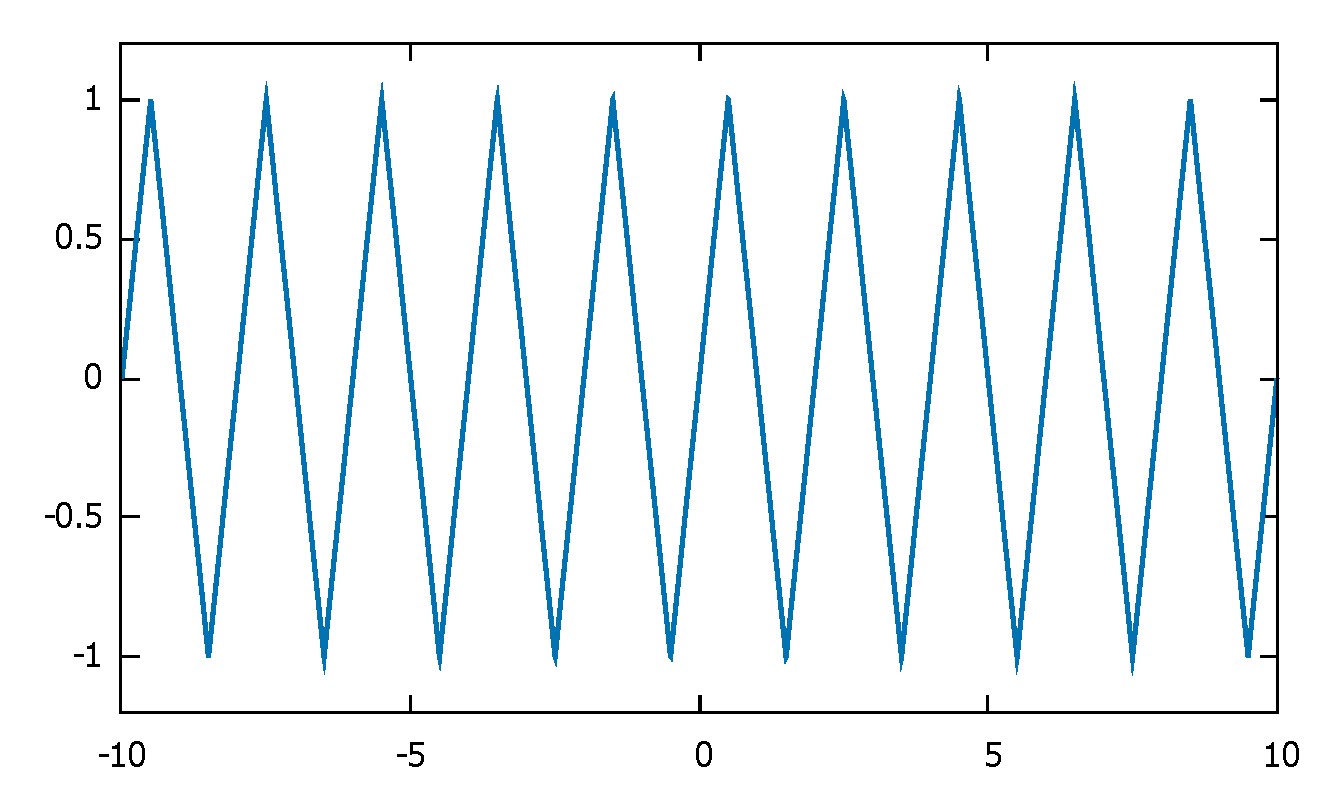
\includegraphics[width=0.4\textwidth]{Abb/dreieck.pdf}
                \caption{Rechtecksfunktion}
                \label{dreieck}
                \vspace{10pt}
            \end{wrapfigure}

Die Dreiecksfunktion ist gegeben durch
                \begin{align*}
                   g(t) = \begin{cases}
                    -2(x+1) & \text{für } -1   < t < -0,5 \\
                    2x      & \text{für } -0,5 < t <  0,5 \\
                    2(x+1)  & \text{für } 0,5  < t <  1
                        \end{cases}
                \end{align*}
auch hier mit periodischer Fortsetzung.
Wiederum müssen die Koeffizienten berechnet werden:
                \begin{itemize}
                   \item es handelt sich um eine ungerade Funktion, also $a_k = 0$
                   \item die $b_k$ ergeben sich zu:
                        \begin{align*}
                            b_k &= \int_{-1}^{-1/2} -2(x+1) \sin(\omega_k t) \dt
                            + \int_{-1/2}^{1/2} 2 \, x \sin(\omega_k t) \dt
                            + \int_{1/2}^{1} 2(1-x) \sin(\omega_k t) \dt \\
                            &= \dots = \frac{4}{\pi^2 k^2}  
                             \left(
                                2 \sin \left( \frac{\pi \,k}{2} \right)
                                - \sin(\pi \, k)
                             \right)
                        \end{align*} 
                \end{itemize}
Die Fourierreihe ergibt sich also zu:
                \begin{align*}
                   g(t) = \sum_{k=0}^\infty \frac{4}{\pi^2 k^2} 
                    \left(
                        2 \sin \left( \frac{\pi \, k}{2} \right)
                        - \sin(\pi \, k) 
                    \right) \cdot \sin(\pi \, k \, t) 
                \end{align*}
                \begin{figure}[htbp]
                  \begin{minipage}{0.45\textwidth}
                   \centering
                    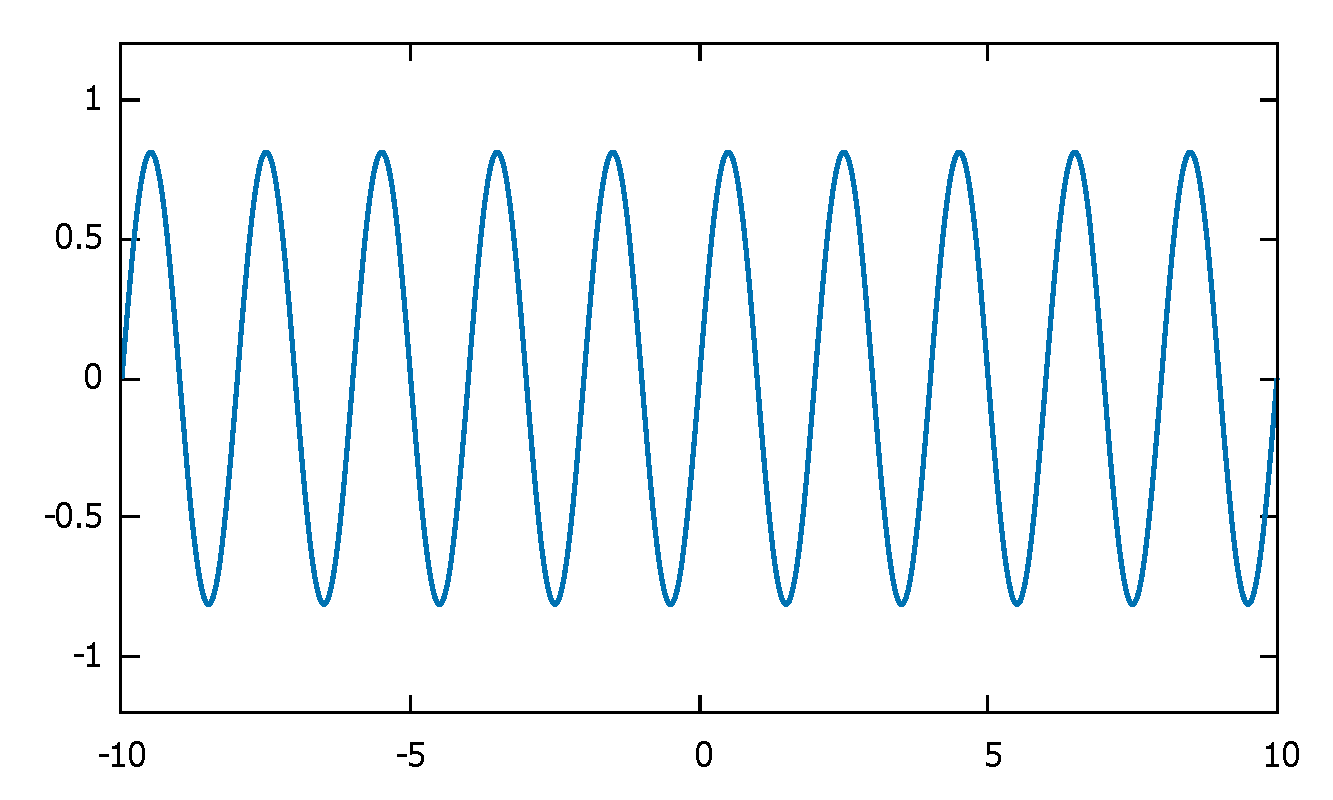
\includegraphics[width=0.9\textwidth]{Abb/dreieck_1}
                    \caption{Die Dreiecksfunktion bis zum 1. Summanden entwickelt}
                    \label{dreieck_1}
                  \end{minipage}\hfill
                  \begin{minipage}{0.45\textwidth}
                   \centering
                    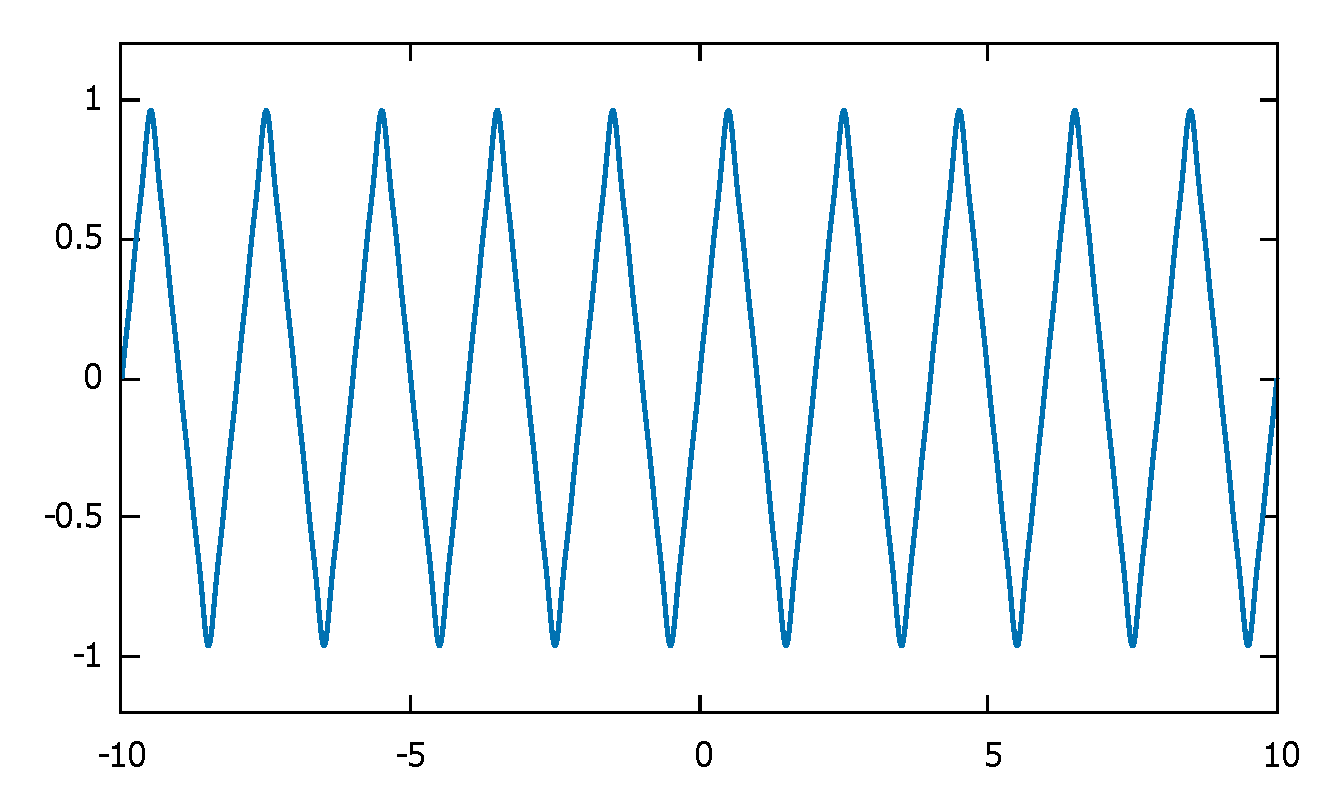
\includegraphics[width=0.9\textwidth]{Abb/dreieck_10.pdf}
                    \caption{Die Dreiecksfunktion bis zum 10. Summanden entwickelt}
                    \label{dreieck_10}
                  \end{minipage}
                \end{figure}
Für Abbildung \ref{dreieck} wurde nur bis zum 1000. Summenglied geplottet. Man sieht
also, dass diese Funktion auch mit weniger Rechenaufwand gut genähert werden kann.
Bei sehr kleinen Ordnungen ist lediglich die Spitze, wie in Abbildung \ref{dreieck_10}
und vor allem in \ref{dreieck_1} zu sehen, noch sehr rundlich.

        \subsection*{Fouriertransformation}
Die Fouriertransformation stellt den Übergang der diskreten Fourierreihe zum
kontinuierlichen Integral dar. Diese erlaubt weiter die Darstellung nicht-periodischer
Funktionen. Für alle integrierbaren Funktionen ist sie definiert als
                \begin{align*}
                   F(f)(k) &= \frac{1}{(2\pi)^{n/2}} \int_{\mathbb{R}^n}
                    f(x) \cdot e^{-ikx} \dx & &\text{\textbf{Hintransformation}}\\
                    f(x) &= \frac{1}{(2\pi)^{n/2}} \int_{\mathbb{R}^n}
                    F(f)(k) \cdot e^{-ikx} \dk & &\text{\textbf{Rücktransformation}}
                \end{align*}
Durch die Fouriertransformation lässt sich eine Funktion über eine ihr zugehörige
andere Variable darstellen. Beispiele hierfür sind Ort $x$ und Wellenzahl $k$,
oder Zeit $t$ und Frequenz $\omega$.

    \section{Beugung}
In der Holografie natürlich ein weiteres Thema ist die Beugung, insbesondere der 
Zusammenhang mit der Fouriertransformation. \emph{Beugung} und \emph{Diffraktion} 
beschreibt die Ablenkung beliebiger Wellen an einem Hindernis.

        \subsection*{Das Beugungsintegral}
Man betrachte an einer Öffnung $\sigma$, die an der Stelle z=0 in der x-y-Ebene steht,
 eine Feldamplitude der Form
    \[
        E_s (x,y) = E_0 (x,y) \cdot e^{i\phi(x,y)}
    \]
Jedes Stück der Fläche strahlt nach dem Huygen'schen Prinzip nun Kugelwellen ab, 
die an einem Punkt $P(x',y')$ einen infinitesimalen Beitrag 
    \[
        \text{d}E_p = C \cdot \frac{E_s \text{d}\sigma}{r}\, e^{ikr}
    \]
zur Feldamplitude beitragen. $\displaystyle C = i \cdot \frac{\cos(\Theta)}{\lambda}$
ist hierbei ein Vorfaktor. Integration über die Öffnung ergibt nun das 
\emph{Fresnel-Kirchhoff'sche Beugungsintegral}
    \[
        E_p = \int \int C \cdot E_s \frac{e^{ikr}}{r} \dx \, \text{dy}
    \]

        \subsection*{Fresnel- und Frauenhofernäherung im Fernfeld}
Zur Vereinfachung dieses Integrals können nun verschiedene Näherungen gemacht werden. \\
Der Abstand zwischen beiden Schirmen sei nun sehr groß im Vergleich 
zur Ausdehnung der Öffnung. Durch diese Annahme ist eine Taylorentwicklung des Abstands
des Ursprungs der Kugelwelle und des Beobachtungspunktes $\vec{r}$ sinnvoll:
\[
    r = \sqrt{z_0^2 + (x-x')^2 + (y-y')^2} \approx z_0 \cdot \left( 1 + 
    \frac{(x-x')^2}{2\,z_0^2}) + \frac{(y-y')^2}{2 \, z_0^2} + \dots \right)
\]
Die quadratischen Terme des Abstands im Nenner des Beugungsintegrals können
hierbei, je nach Phase, vernachlässigt werden. Das Beugungsintegral ergibt sich
in der sog. \emph{Fresnel-Fernfeldnäherung} zu
\[
    E(x',y',z_0) = i \cdot \frac{e^{ikz_0}}{\lambda \, z_0} 
    = \int \int E_s(x,y) \cdot \exp(
        \frac{-ik}{2\,z_0} \left((x-x')^2 + (y-y')^2\right)
    ) \dx \, \text{dy}
\]
Sind die Abmessungen der beugenden Öffnung nun sehr klein im Vergleich zum 
Schirmabstand $z_0$, so kann man zusätzlich die quadratischen Terme $x^2, \; y^2$ 
in der Phase des Beugungsintegrals vernachlässigen
\[
    r \approx z_0 \, \left( 1 - \frac{xx'}{z_0^2} - \frac{yy'}{z_0^2} 
        + \frac{x'^2+y'^2}{2\,z_0^2}
        \right)
\]
Somit ergibt sich für das Beugungsintegral in der \emph{Frauenhofer-Fernfeldnäherung}
\[
    E(x',y',z_0) = A(x',y',z_0) \cdot \int \int E_s(x,y) \cdot
    \exp(\frac{ik}{z_0}(xx'+yy')) \dx \, \text{dy}
\]

    \subsection*{Zusammenhang mit der Fouriertransformation}
Die Feldverteilung an der Blendenöffnung kann, über die einfallende Feldamplitude 
$E_e(x,y)$ moduliert, durch die Transmissionsfunktion der Blende $\tau(x,y)$ beschreiben 
\[
    E_s(x,y) = E_e(x,y) \cdot \tau(x,y)
\]
Wird nun das Beugungsintegral in der Frauenhofernäherung betrachtet, so 
entspricht die Feldverteilung auf dem Schirm $E(x',y',z_0)$ der zweidimensionalen 
Fouriertransformierten der Feldverteilung $E_s(x,y)$ an der beugenden Öffnung.
Dieser Befund wird im Verlaufe des Versuches im Rahmen der \emph{Fourieroptik}
benutzt, um die Bilder einiger Proben zu modulieren.

        \subsection*{Bragg-Beugung}
Die Bragg-Beugung beschreibt die Interferenz eines an einem dreidimensionalen 
Gitter gestreuten Lichtstrahls. Ein wichtiges Resultat ist hier der Zusammenhang 
zwischen Einfallswinkel und Wellenlänge des Strahls, die sog. \emph{Bragg-Bedingung}.
\[
    2\,d\sin(\theta) = m \, \lambda
\]
    \begin{figure}
        \centering
        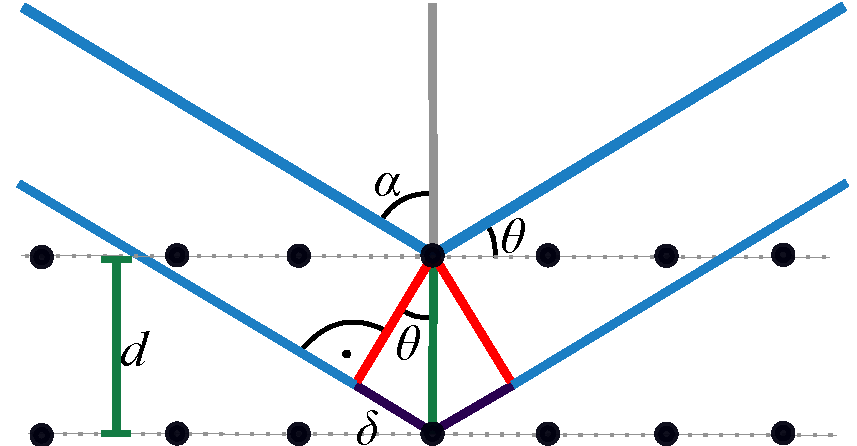
\includegraphics[width=0.7\textwidth]{Abb/Bragg.pdf}
        \caption{Bragg-Beugung}
    \end{figure}

    \section{Frequenzfilterung}
Mit der im vorherigen Abschnitt erwähnten \emph{Fourieroptik}, können die 
\emph{Raumfrequenzen} eines Bildes gefiltert werden. Die Raumfrequenzen sind durch
\[
    \nu_x = \frac{kx'}{z_0}, \quad \nu_y = \frac{ky'}{z_0}
\]
definiert. Die Fouriertransformation in der Fernfeldnäherung transformiert die 
Welle zwischen $x \leftrightarrow \nu_x$ und $y \leftrightarrow \nu_y$.
Bei der Raumfrequenzfilterung wird nun ein Teil dieser Frequenzen 
unterdrückt. 
    \begin{figure}[H]
        \centering
        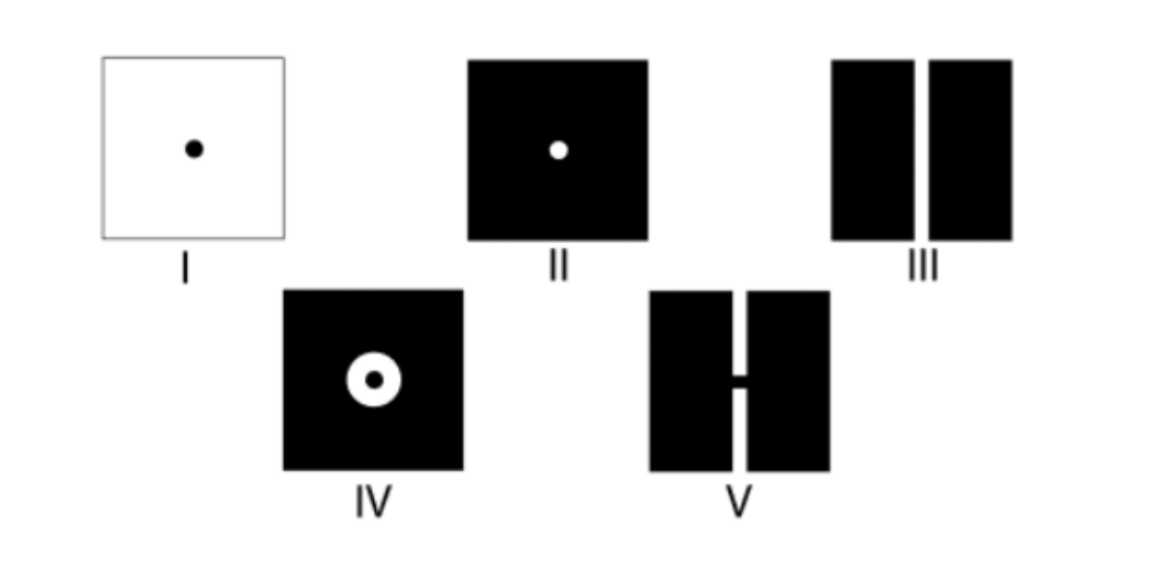
\includegraphics[width=0.6\textwidth]{Abb/filter.PNG}
        \caption{Verschiedene Arten von Raumfrequenzfilterdias
                 \textit{Quelle: Holographie Protokoll, Fischer, Schauer, 2012}
                }
        \label{filter}
    \end{figure}
In obiger Abbildung sind einige Arten von Filtern zu sehen.
    \begin{itemize}
        \item[I] \textbf{Hochpass:} Die Schwärzung in der Mitte des Dias 
        führt zu einer Absorption der tiefen Raumfrequenzen.
        \item[II] \textbf{Tiefpass:} Die Schwärzung des Außenbereiches
        führt zur alleinigen Transmission der tiefen Frequenzen
        \item[III] \textbf{Richtungsfilter:} Hier wird nur eine bestimmte
        Richtung transmittiert.
        \item[IV] \textbf{Bandpass:} Kombination aus Hoch- und Tiefpass
        \item[V] \textbf{Hochpass mit Richtungsfilter:} Kombination aus I und III
    \end{itemize}

    \section{Holographie}
Ein Hologramm erlaubt, zusätzlich zur Intensitätsverteilung, auch die Speicherung
der Phaseninformation der einfallenden Wellen. Im Gegensatz zum Foto werden so
auch Informationen über die Entfernungen der einzelnen Punkte im Raum erfasst.\\
Die Aufnahme eines Hologramms läuft folgendermaßen ab:
Das Objekt wird mit einer kohärenten monochromatischen Lichtquelle beleuchtet. 
Die reflektierte Welle, genannt Objektwelle, wird anschließend auf dem Film mit der 
Referenzwelle überlagert. Das so entstehende Interferenzmuster enthält 
Phaseninformationen.
Siehe dazu Abbildung \ref{holo1}.
\begin{figure}
   \centering
   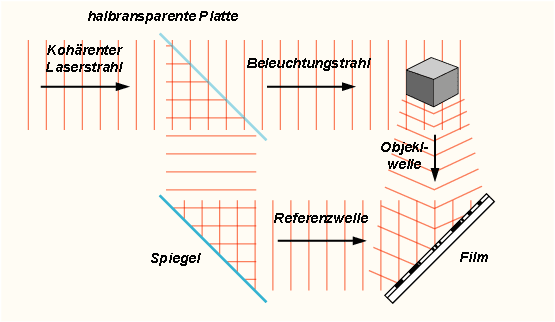
\includegraphics[width=0.6\textwidth]{Abb/holo_ablauf.png} 
   \caption{Ablauf einer holografischen Aufzeichnung}
   \label{holo1}
\end{figure}
Im Rahmen dieses Versuches wird ein Transmissionhologramm, das Fresnel-Holografie,
und ein Reflexionshologramm, das Weißlichthologramm, aufgenommen.
    \begin{itemize}
        \item \textbf{Transmissionshologramm:} Objekt- und Referenzwelle 
        laufen von gleicher Seite auf den Film ein; bei Rekonstruktion 
        läuft Referenzwelle durch den Film hindurch, sodass durch die 
        Modulierung ebendieser die ursprüngliche Objektwelle entsteht
        \item \textbf{Reflexionshologramm:} Wellen laufen aus unterschiedlichen
        Richtungen auf Film ein; Hologramm kann später durch (Bragg-)Reflexion
        einer einlaufenden Welle aus Richtung der Referenzwelle sichtbar gemacht werden
    \end{itemize}

        \subsubsection*{Denisjuk-Hologramm}
Das Denisjuk-Hologramm ist ein Reflexionshologramm und lässt sich durch die
Einstrahlung von weißem Licht rekonstruieren, weshalb es auch Weißlichthologramm
genannt wird. Der Aufbau, in Abbildung \ref{holo2} zu sehen, ist sehr einfach.
\begin{figure}[H]
   \centering
   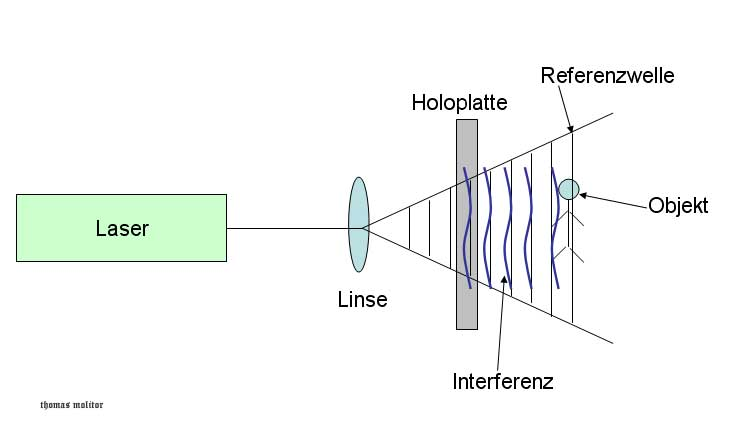
\includegraphics[width=0.8\textwidth]{Abb/denisjuk.jpg} 
   \caption{Aufnahme eines Denisjuk-Hologramms}
   \label{holo2}
\end{figure}
Die Referenzwelle wird von hinten auf die Fotoplatte gestrahlt, während das Objekt 
vor der Fotoplatte steht. Die reflektierte Objektwelle interferiert mit der
Referenzwelle. Die durch diese Interferenz hervorgerufenen lokalen 
Intensitätsverteilungen werden im Film durch unterschiedlich starke Schwärzung
gespeichert. \\

        \subsection*{Fresnel-Hologramm}
Der Aufbau zur Aufnahme eines Fresnel-Hologramms ist in Abbildung \ref{holo1}
zu sehen. Hier treffen die Objekt- und Referenzwelle von der gleichen Seite
auf die Fotoplatte.\\
Zur Rekonstruktion ist es notwendig die Referenzwelle wieder auf den Film
einzustrahlen, was das arbeiten mit Transmissionshologrammen umständlich macht.